%!TEX root = rapport.tex

% \textcolor{navyblue}{\section{Existing visualizations in lambda theory}}
\textcolor{newblue}{\section{Evaluation of existing visualizations in lambda theory}}
According to our research, there does not exist anything exactly similar to our theses exist. There does on the other hand exist visualizations of other lambda-related areas. In this section we will discuss these.

There are numerous examples where a lambda term or a given reduction for a lambda term has been visualized. We have in in just a few hours of research found XX examples of this [See appendix A].

What differentiates these examples from this project is mainly two things:
\begin{itemize}
	\item It is currently not possible to get a complete overview of all the reductions and thereby get an understanding of how the lambda term evaluate over time.
	\item Secondly, non existing visualizations has been capable of doing it beautifully.
\end{itemize}

We will in the rest of this chapter describe three of these examples, which we have selected to be the most interesting.

\subsection{Alligator Eggs -  A Puzzle Game by Bret Victor}

\begin{figure}
	\begin{center}
   		
\includegraphics[scale=0.5]{images/AlligatorEggs.png}
		\caption{Alligator Eggs -  A Puzzle Game}
	\end{center}
\end{figure}

The ``Alligator Eggs -  A Puzzle Game'' \cite{Alligator} is a fun and children-like way of visualizing the computation of a lambda term. It self and is not directly related to our thesis concerning evaluation of the $\beta$-reduction-graphs of the lambda term.\\

The theory in this game is based on the untyped lambda calculus. The game rules is defined according to the following:
\begin{enumerate}
	\item A hungry alligator is a lambda abstraction
	\item An old alligator is parentheses
	\item Eggs are variables
	\item The eating rule corresponds to a $\beta$-reduction
	\item The color rule corresponds to alpha-conversion
	\item The old age rule says that if a pair of parentheses contains a single term, the parentheses can be removed\\\\
\end{enumerate}

In the example below we the eating rule in use. The green alligator will whatever is in front of it. In this case it will eat the yellow alligator and its yellow egg. After the green alligator has eaten the yellow alligator and egg it will die and its egg will hatch into what it has eaten. The miracle of life, as the author calls it. This little episode is, as stated in the definition, corresponding to a $\beta$-reduction. 

\begin{figure}
	\begin{center}
		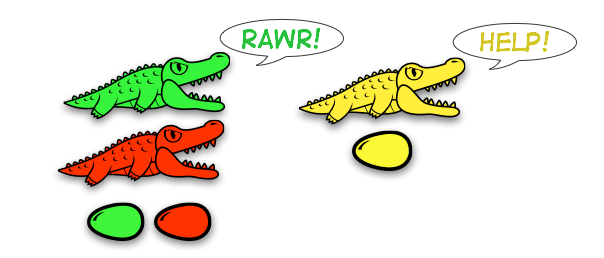
\includegraphics[scale=0.5]{images/alligatorEat.png}
		\caption{A reduction visualized as an alligator eating}	
	\end{center}
\end{figure}

The ``Alligator Eggs -  A Puzzle Game'' does not deal with the same lambda theory as we do in our theses. It does although deal with being visually attractive.

The ``Alligator Eggs -  A Puzzle Game'' has also been implemented in a tool using Java. \cite{AlligatorTool}


\subsection{Lambda Animator by Mike Thyer}
The ``Lambda Animator'' is a representation of lambda expressions in tree form. It is implemented in Java and available online via a Java Applet.

\begin{figure}
	\begin{center}
		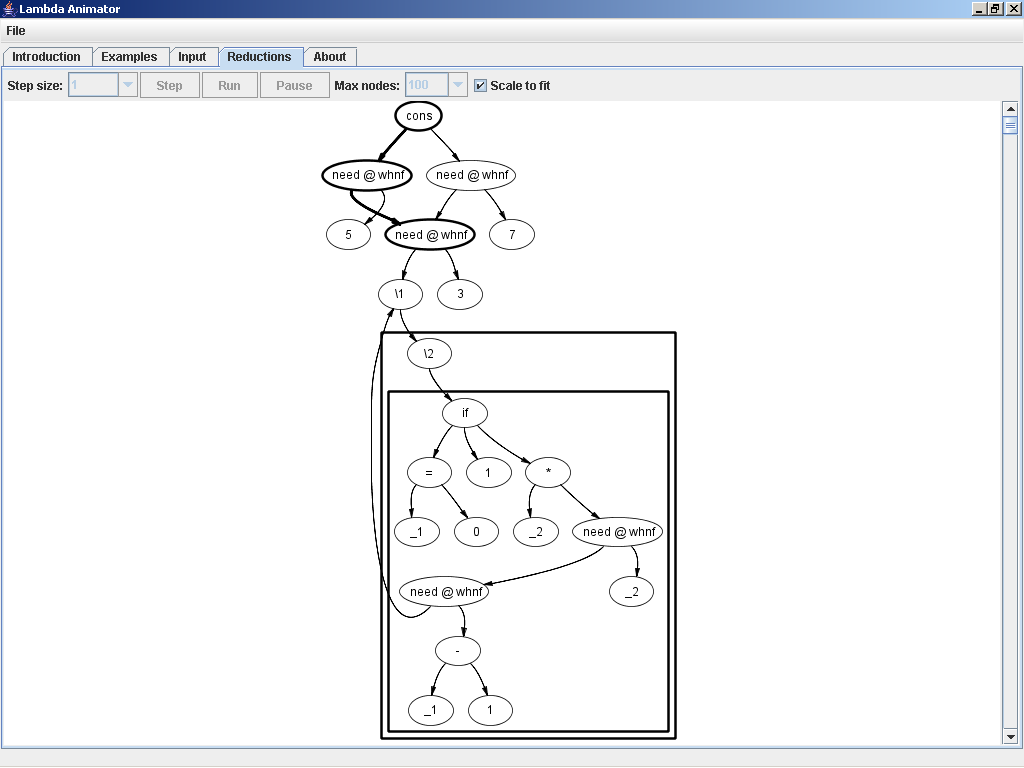
\includegraphics[scale=0.35]{images/lambdaAnimator.png}
		\caption{Screenshot of the Lambda Annimator tool}	
	\end{center}
\end{figure}

The animator does not seem very smooth and does not produce graphs that are neither pretty or especially informative. It uses extremely simple graphics and does not fulfill our ``pretty'' criteria. The implementation in Java (Applet) is although advantageous in terms of easy access to the tool.